\documentclass[14pt, a4paper]{extreport}
\usepackage[utf8]{inputenc}
\usepackage[russian]{babel}
\usepackage[top=20pt,bottom=70pt]{geometry}
\usepackage{amssymb}
\usepackage{amsmath}
\usepackage{graphicx}
\usepackage{listings}
\usepackage[nottoc]{tocbibind}
\renewcommand*\rmdefault{cmr}
\graphicspath{{.}}
\usepackage[left=2cm,right=2cm,bottom=3cm,top=2cm]{geometry}


\DeclarePairedDelimiter{\abs}{\lvert}{\rvert}

\linespread{1.25}

\begin{document}

\thispagestyle{empty}

\begin{center}
	\ \vspace{-3cm}

	\includegraphics[width=0.5\textwidth]{msu.eps}\\
	{Московский государственный университет имени М.В.~Ломоносова}\\
	Факультет вычислительной математики и кибернетики\\
	Кафедра алгоритмических языков

	\vspace{5cm}

	{\Large Кошовец Олег Игоревич}

	\vspace{1cm}

	{\Large\bfseries
	Разложение матрицы полиномов в произведение элементарных матриц\\}

	\vspace{1cm}

	{\large ВЫПУСКНАЯ КВАЛИФИКАЦИОННАЯ РАБОТА}
\end{center}

\vfill

\begin{flushright}
	\textbf{Научный руководитель:}\\
	Профессор д.ф.-м.н.\\
	С.А.Абрамов
\end{flushright}

\vfill


\begin{center}
	Москва, 2018
\end{center}

\newpage
\renewcommand{\contentsname}{Содержание}
\tableofcontents
\clearpage
\newpage

\chapter{Аннотация}
	В данной работе рассматриваются полиномиальные матрицы от одной и нескольких переменных
	и исследуются их разложения в элементарные матрицы. Приводится исследование свойств матриц полиномов
	от одной и нескольких переменных, алгоритм разложения матриц полиномов от одной переменной,
	а также относится написанная для среды компьютерной алгебры Maple программа для разложения
	матриц полиномов от одной переменной.\\
	Результаты данной работы могут быть использованы для дальнейшей работы с полиномиальными матрицами
	и матрицами дифференциальных операторов.

\chapter{Введение}
	Иногда при решении систем дифференциальных уравнений можно установить ряд
	свойств решений, исследуя только матрицы дифференциальных операторов,
	которые описывают систему.
	\\
	Условие разложимости матрицы дифференциальных операторов в произведение
	элементарных матриц является \cite{miyake} признаком голоморфности решений.

	\section{Системы дифференциальных уравнений}
	Пусть $A(x;D) = (a_{ij}(x;D))_{1 \leq i, j \leq N}$ - система обыкновенных
	дифференциальных операторов с голоморфными коэффициентам из $\Omega \subset C$,
	где $D = d/dx$. Пусть $T = (t_1,...,t_n)$ - неотрицательные целые числа. \\
	Тогда можно поставить задачу Коши $(A(x;D), T)$ следующим образом:

	\begin{equation}
	\label{dif:system}
	\begin{aligned}
		& \sum\limits_{j=1}^N a_{ij}(x;D)u_j(x) = f_i(x), & 1 \leq i \leq N,\\
		& D^ku_i(x_0) = w_{i, k} \in \mathbb{C}, & 0 \leq k < t_i,  & 1 \leq i \leq N, & x_0 \in \Omega\\
	\end{aligned}
	\end{equation}

	\section{Свойства решений}
	В работе \cite{miyake} Масатаке Мияке приведены и доказаны теоремы, согласно которым система \ref{dif:system}
	имеет голоморфные решения в каждой точке $x_0 \in \Omega$ тогда и только тогда,
	когда система дифференциальных операторов $A(x;D)$ может быть разложена
	в произведение элементарных матриц. \\\\

\chapter{Постановка задачи}
	Работа с произвольной системы дифференциальных операторов в контексте разложения ее
	в произведение элементарных матриц довольно нетривиальна. Поэтому здесь будет
	рассматриваться упрощение: работа с матрицами полиномов.\\
	Целью данной работы является исследование разложения матриц полиномов от одной и нескольких
	переменных в произведение элементарных матриц, разработка алгоритмов для разложения матриц и
	разработка програмы для системы компьютерной алгебры Maple, производящей это разложение.

\chapter{Обзор существующих решений}
	На момент написания этой работы мною не было найдено каких-либо материалов, посвященных этой задаче.
	В\ "Теории матриц"\ \cite{gantmaher} был изложен теоретический базис, стоящий за элементрными матрицами,
	на основании которого были проведены исследования.\\

	\section{Полиномиальные матрицы}
	Полиномиальной матрицей называется матрица $A(x)$, элементами которой являются полиномы
	$a_{ij}(x)$.\\
	Пусть есть матрица полиномов над действительными числами $A$
	\[
		\begin{bmatrix}
			a_{11} & a_{12} & \dots & a_{1n} \\
			a_{21} & a_{22} & \dots & a_{2n} \\
			\vdots & \vdots & \ddots & \vdots \\
			a_{m1} & a_{m2} & \dots & a_{mn}
		\end{bmatrix}
	\]
	Все последующие рассуждения без изменений проводятся и для случая комплексных чисел, но здесь
	для удобства будут рассматриваться действительные числа.

	\section{Канонический диагональный вид}
	Полиномиальная матрица называется
	канонической диагональной, если она имеет вид
	\[
		\begin{bmatrix}
			a_{1} & 0 & \dots & 0 & 0 & \dots & 0 \\
			0 & a_{2} & \dots & 0 & 0 & \dots & 0 \\
			\dots & \dots & \dots & \dots & \dots & \dots & \dots \\
			0 & 0 & \dots & a_{s} & 0 & \dots & 0 \\
			0 & 0 & \dots & 0 & 0 & \dots & 0 \\
			\dots & \dots & \dots & \dots & \dots & \dots & \dots \\
			0 & 0 & \dots & 0 & 0 & \dots & 0
		\end{bmatrix}
	\]
	где элементы $a_i$ делятся без остатка на элементы $a_{1..i-1}$

	\section{Элементарные преобразования матриц}
	К элементарным преобразованиям матриц относят следующие
	\begin{enumerate}
		\item Перестановка двух строк или двух столбцов
		\item Умножение строки или столбца на некоторую отличную от нуля константу $c$
		\item Прибавление к строке или столбцу другой строки или, соответсвтенно, столбца, домноженный на некоторый полином
	\end{enumerate}
	\section{Элементарные матрицы}
		Каждой элементарной операции над матрицей $A$ можно сопоставить матрицу $S$,
		которая при умножении на исходную матрицу слева или справа выполняет нужное
		преобразование. Действия над строками выполняются с помощью умножения слева
		$S*A$, а операции над столбцами - справа $A*S$. Такие матрицы называются
		элементарными.\\
		Для каждого элементарного преобразования существует свой вид элементарных квадратных матриц
		(здесь нижний индекс обозначает номер строки (столбца) матрицы):
		\begin{enumerate}
			\item Операции перестановки $i$ и $j$ строки (столбца) соответствует матрица вида
				\[
					\begin{bmatrix}
						1_1 & \dots & 0 & \dots & 0 & \dots & 0 \\
						\vdots & & \vdots & & \vdots & & \vdots \\
						0 & \dots & 0 & \dots & 1_j & \dots & 0 \\
						\vdots & & \vdots & & \vdots & & \vdots \\
						0 & \dots & 1_i & \dots & 0 & \dots & 0 \\
						\vdots & & \vdots & & \vdots & & \vdots \\
						0 & \dots & 0 & \dots & 0 & \dots & 1_m \\
					\end{bmatrix}
				\]
				Определитель такой матрицы равен -1.
			\item Операции прибавления к $i$ строке (столбцу) $j$ строки (столбца), домноженной на  полинома $b(x)$,
				соответствует матрица вида
				\[
					\begin{bmatrix}
						1_1   & \dots  & \dots & \dots    & 0 \\
						\vdots & \vdots &       & \vdots  & \vdots \\
						\dots & 1_i    & \dots & $b_j(x)$ & \dots \\
						\vdots & \vdots &       & \vdots  & \vdots \\
						0     & \dots  & \dots & \dots    & 1_m \\
					\end{bmatrix}
				\]
				Определитель такой матрицы равен 1.
			\item Операции умножения $i$ строки (столбца) на ненулевую константу $c$ соответствует матрица вида
				\[
					\begin{bmatrix}
						1_1 & \dots & 0      & \dots 0 \\
						0   &       & \vdots & ~~~~     0 \\
						0   & \dots & c_j    & \dots 0 \\
						0   &       & \vdots & ~~~~     0 \\
						0   & \dots & 0      & \dots 1_m \\
					\end{bmatrix}
				\]
				Определитель такой матрицы равен $c$.
		\end{enumerate}
		Любую последовательнось элементарных преобразований можно
		выполнить с помощью последовательного умножения исходной матрицы с нужной
		стороны на соответствующие элементарные матрицы.\\
		Стоит отметить, что определители элементарных матриц представляют собой численные константы.

	\section{Алгоритм приведения}
	В\ "Теории матриц"\ \cite{gantmaher} Гантмахер изложил алгоритм приведения матрицы полиномов
	к каноническому диагональному виду, использующий только элементарные
	преобразования. Алгоритм состоит из нескольких частей.
	\begin{enumerate}
		\item Выделить в матрице элемент наименьшей степени и
			с помощью перестановок строк и столбцов сделать его элементом $a_{11}$
			\[
				\begin{bmatrix}
					a_{11} & a_{12} & \dots & a_{1n} \\
					a_{21} & a_{22} & \dots & a_{2n} \\
					\vdots & \vdots & \ddots & \vdots \\
					a_{m1} & a_{m2} & \dots & a_{mn}
				\end{bmatrix}
			\]
		\item Последовательно вычесть из строк $2..m$ первую строку,
			домноженную на $q_{s1}$, где $a_{s1} = a_{11}q_{s1} + r_{s1}$, получив
			\[
				\begin{bmatrix}
					a_{11} & a_{12} & \dots & a_{1n} \\
					r_{21} & r_{22} & \dots & r_{2n} \\
					\vdots & \vdots & \ddots & \vdots \\
					r_{m1} & r_{m2} & \dots & r_{mn}
				\end{bmatrix}
			\]
		\item Если среди $r_{21..m1}$ есть элементы, не равные тождественно
			нулю, то алгоритм заново применяется к полученной матрице. В итоге
			получаем матрицу вида
			\[
				\begin{bmatrix}
					a_{11} & a_{12} & \dots & a_{1n} \\
					0 & a_{22} & \dots & a_{2n} \\
					\vdots & \vdots & \ddots & \vdots \\
					0 & a_{m2} & \dots & a_{mn}
				\end{bmatrix}
			\]
		\item По аналогии с пунктом 2 поступаем со столбцами, получая матрицу вида
			\[
				\begin{bmatrix}
					a_{11} & r_{12} & \dots & r_{1n} \\
					0 & a_{22} & \dots & a_{2n} \\
					\vdots & \vdots & \ddots & \vdots \\
					0 & a_{m2} & \dots & a_{mn}
				\end{bmatrix}
			\]
		\item Если среди $r_{12..1n}$ есть элементы, не равные тождественно
			нулю, то алгоритм заново применяется к полученной матрице, начиная
			с пункта 4. В итоге получаем матрицу вида
			\[
				\begin{bmatrix}
					a_{11} & 0 & \dots & 0 \\
					0 & a_{22} & \dots & a_{2n} \\
					\vdots & \vdots & \ddots & \vdots \\
					0 & a_{m2} & \dots & a_{mn}
				\end{bmatrix}
			\]
		\item Алгоритм применяется к $(a_{22}..a_{mn})$ подматрице полученной матрицы.
			На выходе получаем каноническую диагональную матрицу.
	\end{enumerate}
	\newpage

\chapter{Исследование и построение решения задачи}
	Не всякую полиномиальную матрицу можно разложить в произведение элементарных.
	Очевидно, что в произведение элементарных матриц невозможно разложить неквадратную матрицу,
	так как все элементарные матрицы квадратные.
	Очевидно, что невозможно разложить вырожденную матрицу, так как определитель любой элементарной матрицы отличен от нуля.
	Таким образом мы уже наложили некоторые ограничения: будем работать только с невырожденными матрицами.\\
	Используя алгоритм из Гантмахера\cite{gantmaher}, можно привести матрицу к каноническому виду с
	помощью элементарных преобразований. Из этого следует, что из канонического
	вида некоторой матрицы можно восстановить ее исходный вид, проведя обратные
	элементарные преобразования в обратном порядке. Таким образом, переделав
	алгоритм из Гантмахера под нашу конкретную задачу, получаем

	\section{Алгоритм разложения для полиномов одной от одной переменной}
	Пусть есть невырожденная матрица полиномов $A(x)$ размера $m*m$
	\[
		\begin{bmatrix}
			a_{11} & a_{12} & \dots & a_{1m} \\
			a_{21} & a_{22} & \dots & a_{2m} \\
			\vdots & \vdots & \ddots & \vdots \\
			a_{m1} & a_{m2} & \dots & a_{mm}
		\end{bmatrix}
	\]
	Пусть матрица $K$ - канонический вид матрицы $A$
	\[
		\begin{bmatrix}
			a_{1} & 0 & \dots & 0 \\
			0 & a_{2} & \dots & 0 \\
			\vdots & \vdots & \vdots & \vdots \\
			0 & 0 & \dots & a_{m} \\
		\end{bmatrix}
	\]
	Тогда
	\begin{equation*}
		(\prod\limits_{i=1}^{q}L_{i})A(\prod\limits_{j=1}^{r}R_{j}) = K
	\end{equation*}
	где $L_{i},R_{j}$ - элементарные матрицы, соответсвующие элементарным преобразованиям,
	приводящим исходную матрицу к каноническому виду.\\
	Учитывая, что
	\begin{equation*}
		K = (\prod\limits_{l=1}^{m}M_{l})E
	\end{equation*}
	где $M_{l}$ - матрицы, описывающие умножения строки на некоторый многочлен, можно записать:
	\begin{equation*}
		\label{final:form}
		A =
		(\prod\limits_{i=1}^{q}L_{q-i}^{-1})
		(\prod\limits_{l=1}^{m}M_{l})
		(\prod\limits_{j=1}^{r}R_{r-j}^{-1})
	\end{equation*}
	где матрицы $L_{i}^{-1},R_{j}^{-1}$ элементарные. Необходимо, чтобы матрицы $M_{l}$ тоже были
	элементарными, а это выполняется не во всякой невырожденной матрице.

	\section{Применимость алгоритма}
	В Гантмахере \cite{gantmaher} приводится доказательство утверждения,
	что любую невырожденную матрицу полиномов от одной переменной $x$,
	определитель которой не зависит от переменной полинома $x$, можно представить
	в виде произведения элементарных матриц. Для изложенного выше алгоритма выполнение этого
	условия означает, что матрицы $M_{l}$ элементарные, так как их произведение \ref{final:form}
	дает невырожденную матрицу, определитель которой не зависит от $x$.\\
	Мы также можем доказать и обратное утверждение: если матрица $A$ полиномов одной переменной может
	быть представлена в виде произведения элементарных матриц, то ее определитель не равен нулю и
	не зависит от $x$.\\
	Доказательство: известно, что определители элементарных матриц не равны нулю и не зависят от $x$.
	Так как определитель произведения равен произведению определителей, определитель матрицы $A$ будет
	произведением ненулевых констант.\\
	Таким образом мы получаем критерий разложимости матрицы полиномов от одной переменной: квадратная матрица может
	быть представлена в виде произведения элементарных матриц тогда и только тогда, когда ее определитель
	не равен нулю и не зависит от переменной полинома $x$.\\
	Полученный алгоритм раскладывает любую квадратную невырожденную матрицу, определитель которой не зависит
	от $x$, в произведение элементарных матриц.

	\section{Разложение матрицы полиномов от нескольких переменных}
	В случае матрицы полиномов от нескольких переменных алгоритм на основе канонического вида матрицы применять уже нельзя,
	так как этот алгоритм требует постоянного выделения полинома наименьшей степени. Для полиномов от нескольких
	переменных не очень понятно, как именно эту степень считать.\\
	Однако в случае полиномов от нескольких переменных по-прежнему верно утверждение, аналогичное доказанному выше:
	если матрица $A$ полиномов многих переменных может
	быть представлена в виде произведения элементарных матриц, то ее определитель не равен нулю и
	не зависит от $x, y, z ...$ - переменных полиномов.


\chapter{Реализация}
	Предложенный выше алгоритм был реализован в системе компьютерной алгебры Maple.\\
	Результатом работы программы является список элементарных матриц, на которые раскладывается исходная,
	а также список условий, которые должны выполняться на области определения переменных.
	\section{Оптимизации}
	Была улучшена логика нахождения обратной матрицы: обратные матрицы
	создавались сразу и укладывались в список в обратном порядке, в то время как
	матрицы для построения псевдоканонического вида не строились вообще.
	\newpage
	\section{Пример}
	На рисунке представлен пример работы готовой программы.\\
	\begin{center}
		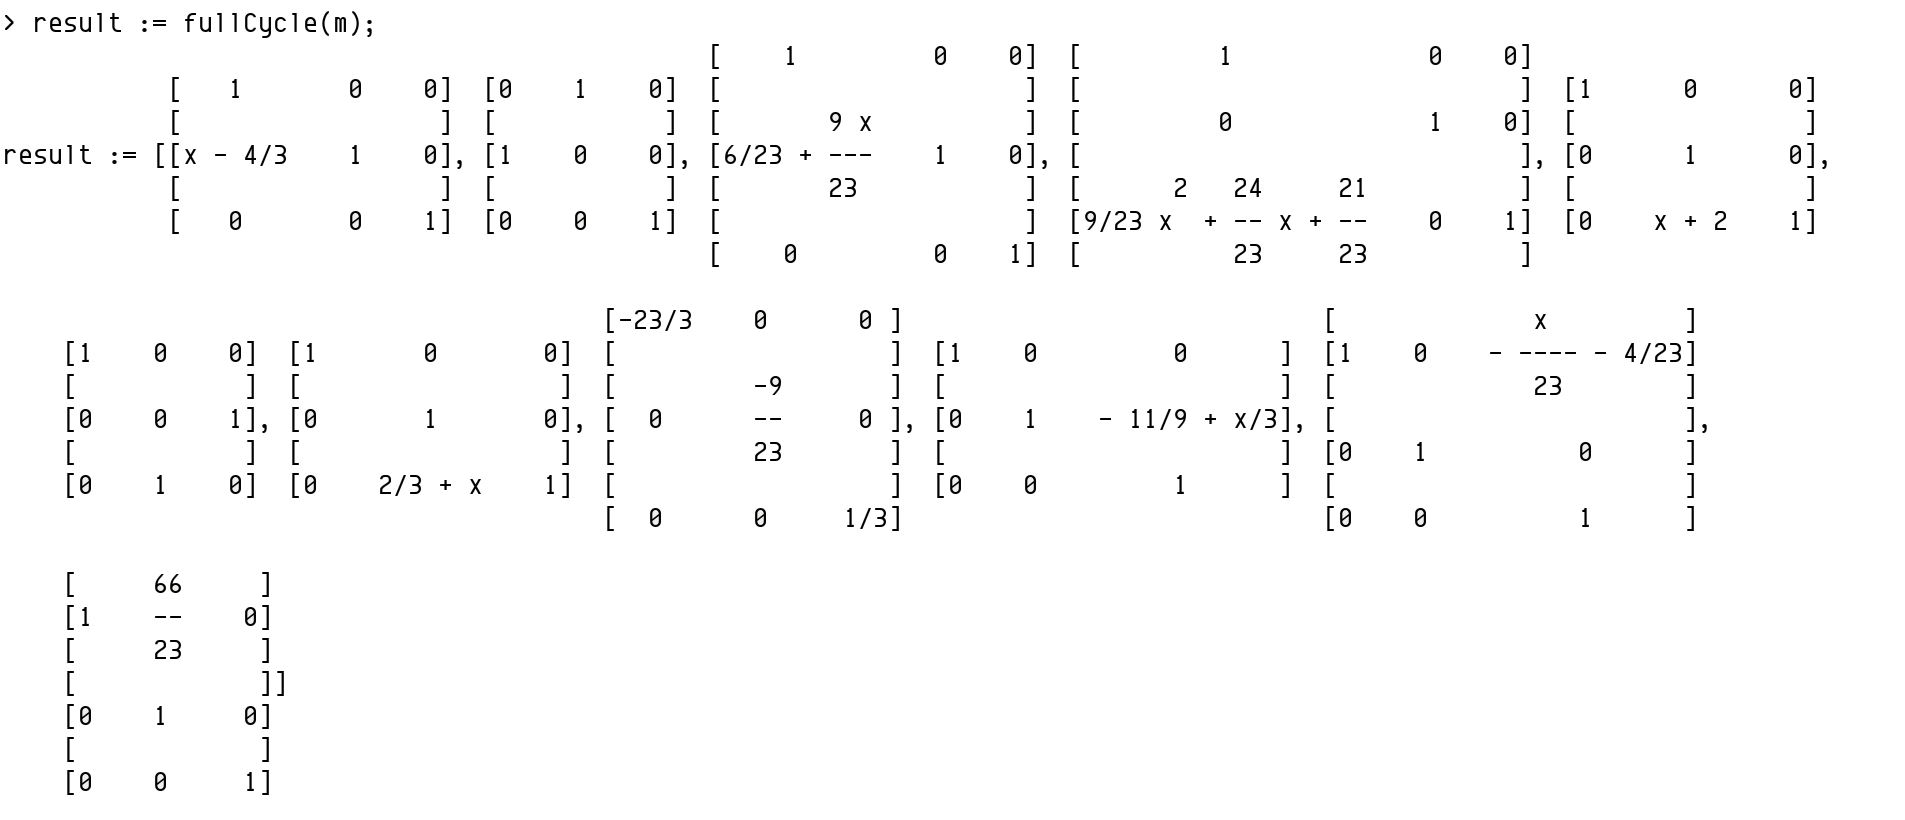
\includegraphics[width=\textwidth]{result2.png}
	\end{center}
\chapter{Итоги}
\section{Результаты}
\begin{enumerate}
	\item Изучена работа \cite{miyake} Мисатаке Мияке, сформулирована задача на ее основе
	\item Изучен алгоритм, представленный в\ "Теории Матриц"\ Гантмахера \cite{gantmaher}
	\item Алгоритм адаптирован для работы с матрицами полиномов от одной переменной.
	\item Алгоритм переделан для работы с матрицами полиномов от нескольких переменных.
	\item Изучена система компьютерной алгебры Maple
	\item Написана программа, производящая разложения матрицы полиномов от нескольких переменных в произведение элементарных матриц
	\item Изучена и освоена верстка в LaTeX
\end{enumerate}
Результаты этой научной работы потенциально могут быть использованы
для решения задач, сформулированных в работе \cite{miyake} Мияке.
\begin{thebibliography}{5}
	\bibitem{gantmaher}
		Ф.Р.Гантмахер
		\textit{"Теория матриц"}
		Издательство “Наука” 1966
	\bibitem{miyake}
		M.Miyake
		\textit{“Remarks on the formulation of the Cauchy problem
		for general system of ordinary differential equations”}
		Tohoku Math. Journal 1979
	\bibitem{maple}
		M.Monogan
		\textit{“Maple 9. Introductory Programming Guide”}
		ISBN 1-894511-43-3
	\bibitem{maplesoft}
		\textit{Maplesoft.com}
	\bibitem{mapleprimes}
		\textit{Mapleprimes.com}
\end{thebibliography}
\end{document}
